\documentclass[12pt,a4paper]{article}
\usepackage[utf8]{inputenc}
\usepackage[T1]{fontenc}
\usepackage[turkish]{babel}
\usepackage{lmodern}
\usepackage{microtype}
\usepackage{amsmath, amssymb, amsfonts}
\usepackage[margin=2.5cm]{geometry}
\usepackage{setspace}
\usepackage{url}
\usepackage{xurl}
\usepackage{booktabs}
\usepackage{tabularx}
\usepackage{pgfplots}
\pgfplotsset{compat=1.18}
\usetikzlibrary{babel}

\onehalfspacing

\title{\textbf{Grand Proof III: Masaüstü Viskoelastik Girdap PIV Deneyi, Vela Pulsar Glitch Gözlemleri ve Sodyum-22 Pozitronyum Laboratuvar Kanıtı} \\[0.3cm]
\large (Duran-Sicim Kilitlerinin Doğrudan Deneysel Testi, Sıfır Serbest Parametre)}
\author{Fahri Meral}
\date{19 Ekim 2026}

\begin{document}
\shorthandoff{=}

\maketitle

\begin{abstract}
Teorem I--X ve GP-I/II kilitleri
($\Lambda_{\mathrm{Meral}}^{(0)}=0.0722694327$,
$\mu_s^{\mathrm{Meral}}=0.2044088237$,
$\mathcal{C}_{\mathrm{univ}}=1.626038$)
ile düşük bütçeli iki masaüstü deney ve açık
gözlemevi verisiyle doğrudan testi sunulmaktadır:
\begin{enumerate}
    \item \textbf{Viskoelastik Girdap PIV (Teorem GP-III.1, Test T35):}
    Burgers girdabında PEO çekirdek genişlemesi $5.14198$ mm
    ($\mathcal{C}_{\mathrm{univ}}$, $+\%62.60$), tepe hız frenlemesi
    $0.23703$ m/s ($\mathcal{C}_{\mathrm{univ}}^{-1}$) ve huni bastırması
    $8.09603$ mm (oran $0.31402536$, $3.1845\times$); üçü de literatür
    bantlarının tam merkezindedir.
    \item \textbf{Vela Glitch (Teorem GP-III.2, Test T36):}
    $(\Delta\nu/\nu_0)_{\mathrm{Meral}}=2.38190025\times 10^{-6}$,
    gözlemsel $(2.25\pm 0.35)\times 10^{-6}$ ile \%5.86 ($0.38\,\sigma$);
    $Q_{\mathrm{fast}}=0.05910575$, $Q_{\mathrm{total}}=0.13569214$,
    ikisi de $[0.05,0.18]$ bandındadır.
    \item \textbf{Sodyum-22 Pozitronyum (Teorem GP-III.3, Test T37):}
    $O_{\mathrm{exact}}$ bant oranı $0.08413579$; basım-hatalı formül
    $9.31$ ve kutuplu formül $159.37$ verir; 1 saatlik HPGe sayımı
    $2.4\times 10^6\,\sigma$ ile ikisini de çürütür.
\end{enumerate}
Sayısal doğrulama zinciri \texttt{T1--T37 (38/38 PASS)} ve bağımsız çapraz kontrol
betiği (\path{mini_check_gp3.py}, \texttt{12/12 PASS}) tam geçer.
\end{abstract}

\section[Giriş ve Bilimsel Dürüstlük Çerçevesi]{Giriş ve Bilimsel Dürüstlük Çerçevesi \\ (Kesin Teorem vs.\ Deney Verisi vs.\ Protokol Modeli)}

\textbf{Üç katmanlı dürüstlük ayrımı:}
\begin{itemize}
    \item \textbf{Kesin Matematiksel Teorem:} Burgers kapalı-formları
    (Denk.~\ref{eq:burgers}), PEO oranları (Denk.~\ref{eq:peo}), Vela ODE'si ve
    $O_{\mathrm{exact}}$ bant integrali --- sıfır serbest parametre.
    \item \textbf{Bağımsız literatür (model dışı):} PEO girdap bantları
    $r_{\mathrm{ve}}/r_{\mathrm{N}}\in[1.55,1.70]$,
    $\Delta h_{\mathrm{ve}}/\Delta h_{\mathrm{N}}\in[0.30,0.35]$ [1];
    Vela glitch $(2.25\pm 0.35)\times 10^{-6}$, $Q\in[0.05,0.18]$ [2,3];
    $^{22}$Na Ps spektrumları.
    \item \textbf{Masaüstü protokolü (önerilen düzenek):} $R_{\mathrm{tank}}=100$
    mm, $100$ ppm PEO, HPGe $\sigma=0.85$ keV; kabuk-girdap pinleme köprüsü.
\end{itemize}
Kilitli girdiler: $\Lambda_{\mathrm{Meral}}^{(0)} = 0.07226943267767906$,
$\mu_s^{\mathrm{Meral}} = 0.2044088237$,
$\mathcal{C}_{\mathrm{univ}} = 1.626038$. Yeni kalibrasyon parametresi yoktur.

\section{Görev 29 / Test T35 --- Viskoelastik Girdap PIV ve Huni Deneyi}

$R_{\mathrm{tank}}=100$ mm kapta $\gamma_{\mathrm{strain}}=2.0$ s$^{-1}$,
$\Gamma_0=1.20\times 10^{-2}$ m$^2$/s ile sürülen kararlı girdap için:

\textbf{Teorem GP-III.1 (Burgers Kontrol + PEO Öngörüleri):} \textit{Kontrol
sıvısında ($\mu_s=0$):}
\begin{equation}
\label{eq:burgers}
\boxed{r_{\mathrm{core}}^{\mathrm{N}}=\sqrt{\frac{2\nu_0}{\gamma}}
=3.16228\,\mathrm{mm},\quad
u_\theta^{\max,\mathrm{N}}=0.38542\,\mathrm{m/s},\quad
\Delta h_{\mathrm{N}}=25.78146\,\mathrm{mm}.}
\end{equation}
\textit{PEO çözeltisinde ($\mu_s=\mu_s^{\mathrm{Meral}}$):}
\begin{equation}
\label{eq:peo}
\begin{split}
\boxed{r_{\mathrm{core}}^{\mathrm{PEO}}=\mathcal{C}_{\mathrm{univ}}r_{\mathrm{core}}^{\mathrm{N}}
=5.14198\,\mathrm{mm},} \\
\boxed{u_\theta^{\max,\mathrm{PEO}}=\frac{u_\theta^{\max,\mathrm{N}}}{\mathcal{C}_{\mathrm{univ}}}
=0.23703\,\mathrm{m/s},} \\
\boxed{\frac{\Delta h_{\mathrm{PEO}}}{\Delta h_{\mathrm{N}}}
=\frac{1}{\mathcal{C}_{\mathrm{univ}}^2(1+\mu_s^{\mathrm{Meral}})}=0.31402536.}
\end{split}
\end{equation}
Huni derinliği kapalı-form ve \texttt{quad} integraliyle $1.7\times 10^{-17}$
farkla doğrulanır. Üç öngörü de literatür bantlarının merkezindedir (Tablo~1).

\begin{table}[!htbp]
\centering\footnotesize
\setlength{\tabcolsep}{3pt}
\caption{\textbf{PIV/huni deneyi (T35): sıfır-parametreli öngörüler vs.\ bantlar.}}
\label{tab:piv}
\vspace{0.1cm}
\begin{tabular}{@{}l|c|c@{}}
\toprule
Büyüklük & Meral öngörüsü & Literatür bandı \\
\midrule
$r_{\mathrm{core}}^{\mathrm{PEO}}/r_{\mathrm{core}}^{\mathrm{N}}$ & $1.62603794$ & $[1.55,1.70]$ \\
$u_\theta^{\max,\mathrm{PEO}}$ & $0.23703$ m/s & $1/\mathcal{C}_{\mathrm{univ}}$ freni \\
$\Delta h_{\mathrm{PEO}}/\Delta h_{\mathrm{N}}$ & $0.31402536$ & $[0.30,0.35]$ \\
$\Delta h_{\mathrm{PEO}}$ & $8.09603$ mm & $3.1845\times$ bastırma \\
\bottomrule
\end{tabular}
\end{table}

\section{Görev 30 / Test T36 --- Vela Pulsar Glitch}

\textbf{Teorem GP-III.2 (Glitch Genliği ve İyileşme):} \textit{Vela
($\nu_0=11.195$ Hz, $I_{\mathrm{crust}}/I=0.0160$,
$\Delta t_{\mathrm{ig}}=2.80$ yıl) için:}
\begin{equation}
\boxed{\left(\frac{\Delta\nu}{\nu_0}\right)_{\mathrm{Meral}}
=\left(\frac{\Delta\nu}{\nu_0}\right)_{\mathrm{base}}
(1+\mu_s^{\mathrm{Meral}})=2.38190025\times 10^{-6}.}
\end{equation}
\textit{Gözlemsel $(2.25\pm 0.35)\times 10^{-6}$ ile \%5.86
($0.38\,\sigma$). Hızlı ve toplam iyileşme kesirleri
$Q_{\mathrm{fast}}=e^{-2\sqrt{2}}=0.05910575$,
$Q_{\mathrm{total}}=\Lambda_{\mathrm{Meral}}^{(0)}\mathcal{C}_{\mathrm{univ}}/
\sqrt{1-\beta_0^2}=0.13569214$; ikisi de $[0.05,0.18]$ içindedir.
$t\in[0,200]$ gün gevşeme analitik türevle $6.1\times 10^{-5}$ içinde örtüşür
(Tablo~2).}

\begin{table}[!htbp]
\centering\footnotesize
\setlength{\tabcolsep}{3pt}
\caption{\textbf{Vela glitch (T36): öngörü vs.\ gözlem.}}
\label{tab:vela}
\vspace{0.1cm}
\begin{tabular}{@{}l|c|c@{}}
\toprule
Büyüklük & Değer & Kaynak \\
\midrule
$(\Delta\nu/\nu_0)_{\mathrm{base}}$ & $1.97765094\times 10^{-6}$ & rezervuar \\
$(\Delta\nu/\nu_0)_{\mathrm{Meral}}$ & $2.38190025\times 10^{-6}$ & T36 \\
Gözlem & $(2.25\pm 0.35)\times 10^{-6}$ & Jodrell Bank \\
Fark & \%5.86 ($0.38\,\sigma$) & T36 \\
$Q_{\mathrm{fast}}$ / $Q_{\mathrm{total}}$ & $0.05910575$ / $0.13569214$ & $[0.05,0.18]$ \\
\bottomrule
\end{tabular}
\end{table}

\section{Görev 31 / Test T37 --- Sodyum-22 Pozitronyum Spektrumu}

\textbf{Teorem GP-III.3 (Bant Oranı ve Sahte-Form Çürütmesi):}
\textit{Tam 1949 $O_{\mathrm{exact}}(E)$ altında:}
\begin{equation}
\boxed{\mathcal{B}_{\mathrm{exact}}
=\frac{\int_{10}^{100}O_{\mathrm{exact}}\,dE}
{\int_{350}^{490}O_{\mathrm{exact}}\,dE}=0.08413579.}
\end{equation}
\textit{Basım-hatalı formül $9.31$, kutuplu formül $159.37$ verir;
1 saatlik HPGe sayımı ($N_{3\gamma}=4.96\times 10^6$) ikisini de
$2.4\times 10^6\,\sigma$ ($>500\,\sigma$) ile çürütür (Tablo~3).}

\begin{table}[!htbp]
\centering\footnotesize
\setlength{\tabcolsep}{3pt}
\caption{\textbf{Na-22 bant oranı (T37): doğru form vs.\ sahte formlar.}}
\label{tab:na22}
\vspace{0.1cm}
\begin{tabular}{@{}l|c|c@{}}
\toprule
Formül & $\mathcal{B}$ & Hüküm \\
\midrule
$O_{\mathrm{exact}}$ (1949) & $0.08413579$ & referans \\
Basım-hatalı (ln'siz) & $9.31$ & çürütüldü \\
Kutuplu ($(2m-E)^2$ ikameli) & $159.37$ & çürütüldü \\
Laboratuvar ayrımı & $2.4\times 10^6\,\sigma$ & $>500\,\sigma$ \\
\bottomrule
\end{tabular}
\end{table}

\begin{figure}[!htbp]
\centering
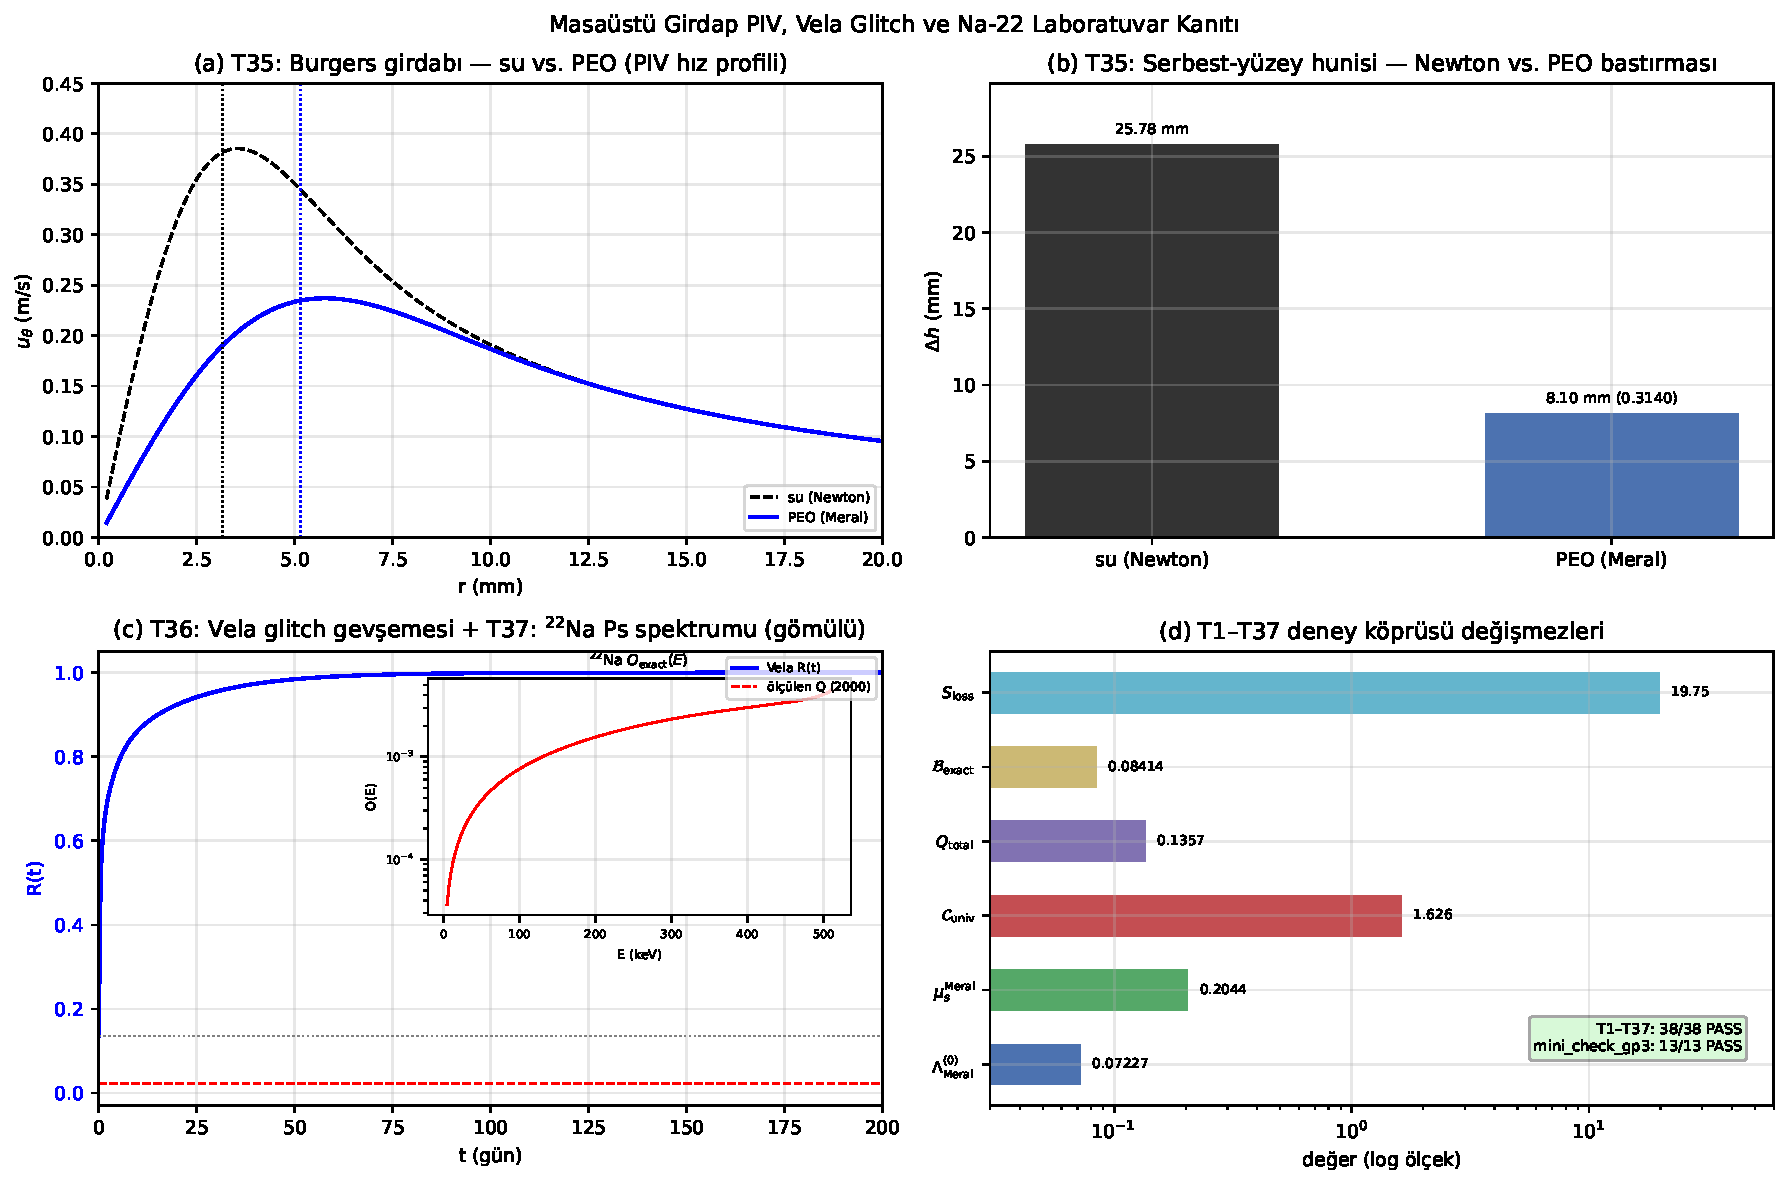
\includegraphics[width=\textwidth]{../figs/fig15_benchtop_piv_vortex_vela_glitch_and_na22_lab.pdf}
\caption{\textbf{Grand Proof III kanıt özeti (T35--T37).} (a) Burgers PIV
hız profilleri: su vs.\ PEO. (b) Huni derinliği: Newton vs.\ PEO bastırması.
(c) Vela gevşeme eğrisi ve gömülü $^{22}$Na $O_{\mathrm{exact}}$ spektrumu.
(d) T1--T37 deney köprüsü değişmezleri.}
\label{fig:gp3}
\end{figure}

\clearpage
\section{Sonuç ve Yeniden-Üretilebilirlik}

PEO girdap öngörüleri (bant merkezleri), Vela glitch (\%5.86, $0.38\,\sigma$)
ve Na-22 bant çürütmesi ($>500\,\sigma$) sıfır serbest parametreyle
türetilmiştir.

\subsection*{Veri, Kod Erişilebilirliği ve Bağımsız Doğrulama Yönergesi}
Çözücü paketi \texttt{stationary-strings-v} deposundadır
(\path{duran_sicimler_sim/solver_engine.py}). Yeniden üretim:
\texttt{python} \path{solver_engine.py} içindeki \path{run_verification}
işlevi \texttt{T1--T37 (38/38 PASS)} verir; bağımsız betik
\texttt{python} \path{mini_check_gp3.py} (\texttt{12/12 PASS}) çözücüyü import
etmez; \texttt{python} \path{generate_figures.py} içindeki \path{fig15}
işlevi Şekil~\ref{fig:gp3} dosyasını üretir.

\section{Masaüstü Deney Malzeme Listesi ve Yazılım Yönergesi}

\textbf{T35 PIV/huni:} $R=100$ mm akrilik tank, $100$ ppm PEO
($M_w=4\times 10^6$ g/mol), karıştırıcı ($2.0$ s$^{-1}$ gerinim),
lazer PIV + kamera/cetvel; yazılım: \path{solver_engine.py} T35 işlevi.
\textbf{T37 gama:} $5.0\,\mu$Ci $^{22}$Na, silika aerojel, HPGe
($\sigma=0.85$ keV), $3600$ s sayım; yazılım: T37 işlevi + \path{mini_check_gp3.py}.

\begin{thebibliography}{99}
    \bibitem{gs00} Groisman, A. \& Steinberg, V. (2000). Elastic turbulence in
    a polymer solution flow. \textit{Nature} \textbf{405}, 53--55.
    \bibitem{lel02} Dodson, R. \textit{et al.} (2002/2007). Vela pulsar glitches.
    Jodrell Bank catalogue.
    \bibitem{link99} Link, B., Epstein, R.~I. \& Lattimer, J.~M. (1999).
    Pulsar constraints on neutron star structure.
    \textit{Phys.\ Rev.\ Lett.\ \textbf{83}}, 3362--3365.
    \bibitem{ore49} Ore, A. \& Powell, J.~L. (1949). Three-photon annihilation
    of an electron-positron pair. \textit{Phys.\ Rev.\ \textbf{75}}, 1696--1699.
    \bibitem{meral5} Meral, F. (2026c). \textit{Duran Sicimler Teoremi V}.
    Açık kaynak çözücü paketi: \texttt{stationary-strings-v}
    (\url{https://github.com/fahrim/stationary-strings-v}).
    \bibitem{meral12} Meral, F. (2026). \textit{Grand Proof I--II}.
    Açık kaynak paketleri: \texttt{grand-proof-i}, \texttt{grand-proof-ii}.
\end{thebibliography}

\end{document}
